\documentclass[14pt,pdf,hyperref={unicode}]{beamer}

% \documentclass[aspectratio=43]{beamer}
% \documentclass[aspectratio=1610]{beamer}
% \documentclass[aspectratio=169]{beamer}

\usepackage{lmodern}

% подключаем кириллицу 
\usepackage[T2A]{fontenc}
\usepackage[utf8]{inputenc}
\usepackage{listings}
\usepackage{graphicx}
\usepackage{hyperref}

% отключить клавиши навигации
\setbeamertemplate{navigation symbols}{}

% тема оформления
\usetheme{CambridgeUS}

% цветовая схема
\usecolortheme{seahorse}

\definecolor{light-gray}{gray}{0.90}

\lstset{basicstyle=\ttfamily,breaklines=true}

\title{Семинар №6}   
\subtitle{ФАКИ 2015}
\author{Бирюков В. А.} 
\date{\today} 
% \logo{
\includegraphics[height=5mm]{images/logo.png}\vspace{-7pt}}

\begin{document}

\lstset{language=C}

% титульный слайд
\begin{frame}
\titlepage
\end{frame} 

\defverbatim[colored]\makeset{
\begin{lstlisting}[language=C++,basicstyle=\ttfamily,keywordstyle=\color{blue}]
void make_set(int X) {
  parent[X] = X;
}
\end{lstlisting}
}

\lstset{
  language=C,                % choose the language of the code
  keywordstyle=\color{blue},
  numbers=none,                   % where to put the line-numbers
  stepnumber=1,                   % the step between two line-numbers.        
  numbersep=5pt,                  % how far the line-numbers are from the code
  backgroundcolor=\color{light-gray},  % choose the background color. You must add \usepackage{color}
  showspaces=false,               % show spaces adding particular underscores
  showstringspaces=false,         % underline spaces within strings
  showtabs=false,                 % show tabs within strings adding particular underscores
  tabsize=2,                      % sets default tabsize to 2 spaces
  captionpos=b,                   % sets the caption-position to bottom
  breaklines=true,                % sets automatic line breaking
  breakatwhitespace=true,         % sets if automatic breaks should only happen at whitespace
}






\section{Строки}
\begin{frame}
\begin{center}
\begin{beamercolorbox}[sep=8pt,center]{part
title}
\usebeamerfont{part title}\insertsection
\end{beamercolorbox}
\end{center}
\end{frame}


\begin{frame}[fragile]
\frametitle{Строки} 
\begin{itemize}
\item Строки в языке C -- на самом деле массивы из элементов типа char
\item Существенное отличие -- в конце строки должен стоять символ '\textbackslash 0'
\item Объявление:
\begin{lstlisting}
char string[10];
\end{lstlisting}
\item Доступ к элементу
(Нумерация в строке тоже начинается с 0):\\
\begin{lstlisting}
printf("%c\n", string[0]);
\end{lstlisting}
\end{itemize}
\end{frame}


\begin{frame}[fragile]
\frametitle{Строки} 
\framesubtitle{Строки в памяти}
\begin{center}
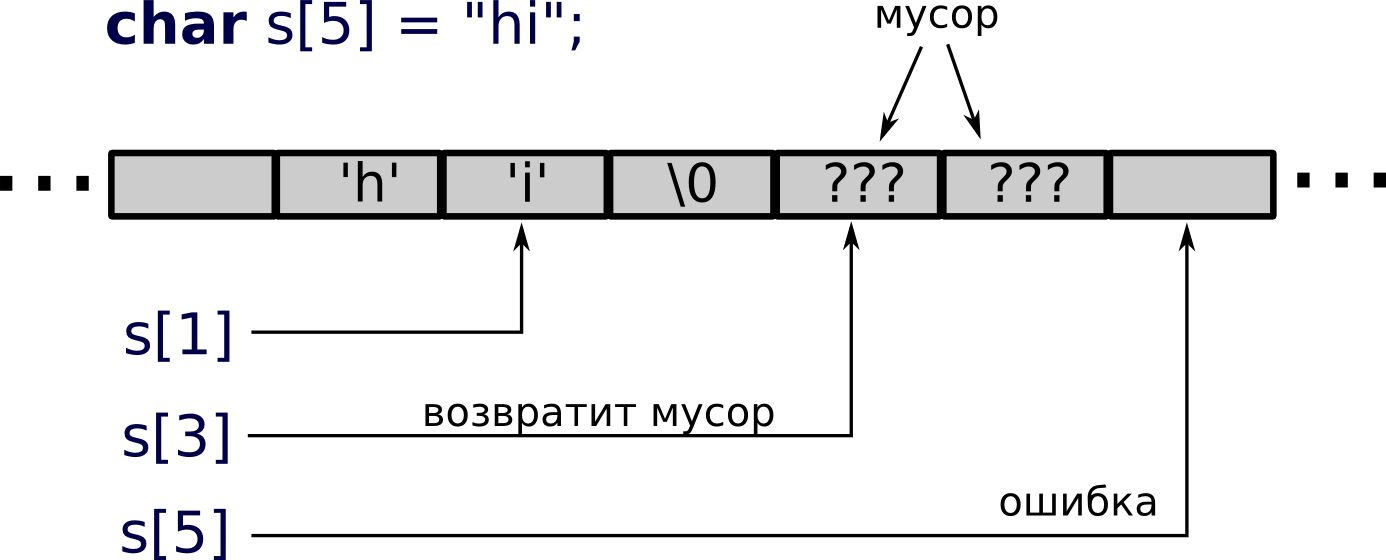
\includegraphics[width=0.95\linewidth]{images/string_in_memory.png}
\end{center}
\end{frame}

\begin{frame}[fragile]
\frametitle{Функции для работы со строками} 
Чтение строки:
\begin{lstlisting}
char string[10];
scanf("%10s", string);
\end{lstlisting}
Длина строки:
\begin{lstlisting}
#include <string.h>
char string[10] = "hello";
int n = strlen(string);
\end{lstlisting}
\end{frame}

\begin{frame}[fragile]
\frametitle{Функции для работы со строками} 
\begin{lstlisting}
#include <string.h>
char s1[10] = "hi";
char s2[10] = "world";
\end{lstlisting}
Копирование строки s2 в строку s1:
\begin{lstlisting}
strcpy(s1, s2);
\end{lstlisting}
Конкатенация строки s2 в строку s1:
\begin{lstlisting}
strcat(s1, s2);
\end{lstlisting}
\end{frame}

\begin{frame}[fragile]
\frametitle{Функции для работы со строками} 
\begin{lstlisting}
#include <string.h>
char s1[10] = "hi";
char s2[10] = "hello";
\end{lstlisting}
Сравнение строк s1 и s2:
\begin{lstlisting}
strcmp(s1, s2);
\end{lstlisting}
Возвращает указатель на первое вхождение строки s2 в строку s1:
\begin{lstlisting}
strstr(s1, s2);
\end{lstlisting}
\end{frame}


\section{Структуры}
\begin{frame}
\begin{center}
\begin{beamercolorbox}[sep=8pt,center]{part
title}
\usebeamerfont{part title}\insertsection
\end{beamercolorbox}
\end{center}
\end{frame}




\begin{frame}[fragile]
\frametitle{Структуры} 
\begin{itemize}
\item Структура -- это композитный тип данных, группирующий, без сокрытия набор значений \\
\item 
\begin{lstlisting}[language=C++,basicstyle=\ttfamily,keywordstyle=\color{blue}]
struct tag_name {
   type1 member1;
   type2 member2;
   /* ... */
};
\end{lstlisting}
\end{itemize}
\end{frame}


\begin{frame}[fragile]
\frametitle{Структуры} 
\framesubtitle{Пример} 
Описание структуры:
\begin{lstlisting}[language=C++,basicstyle=\ttfamily,keywordstyle=\color{blue}]
struct account {
   int account_number;
   char first_name[30];
   char last_name[50];
   float balance;
};
\end{lstlisting}
Объявление структуры:
\begin{lstlisting}[language=C++,basicstyle=\ttfamily,keywordstyle=\color{blue}]
struct account ac1;
\end{lstlisting}
\end{frame}

\begin{frame}[fragile]
\frametitle{Структуры} 
\framesubtitle{Пример} 
Инициализация структуры:
\begin{lstlisting}[language=C++,basicstyle=\ttfamily,keywordstyle=\color{blue}]
struct account ac1 = {1, "Ivan", "Ivanov", 1000.0};
\end{lstlisting}
Доступ к элементу структуры(оператор .):
\begin{lstlisting}[language=C++,basicstyle=\ttfamily,keywordstyle=\color{blue}]
ac1.first_name = "Petr";
ac1.balance += 100;
printf("%s has %.2f roubles\n", ac1.last_name, ac1.balance);
\end{lstlisting}
\end{frame}


\begin{frame}[fragile]
\frametitle{Typedef} 
\begin{itemize}
\item Typedef -- ключевое слово в языке C \\
\item Используется для того, чтобы дать типу новое имя \\
\item 
\begin{lstlisting}[language=C++,basicstyle=\ttfamily,keywordstyle=\color{blue}]
typedef unsigned long long ull;
\end{lstlisting}
\item 
\begin{lstlisting}[language=C++,basicstyle=\ttfamily,keywordstyle=\color{blue}]
typedef struct {
   int    account_number;
   char   first_name[30];
   char   last_name[50];
   float  balance;
} account;
\end{lstlisting}
\end{itemize}
\end{frame}

\begin{frame}[fragile]
\frametitle{Структуры и функции} 
\framesubtitle{Передача структур по значению} 

\begin{lstlisting}[language=C++,basicstyle=\ttfamily,keywordstyle=\color{blue}]
void print(account ac)
{
    printf("%s has %.2f roubles\n", ac.last_name, ac.balance);
}
\end{lstlisting}
\end{frame}



\begin{frame}[fragile]
\frametitle{Структуры и функции} 
\framesubtitle{Передача структур с помощью указателей} 

\begin{lstlisting}[language=C++,basicstyle=\ttfamily,keywordstyle=\color{blue}]
void print(account * ac)
{
    printf("%s has %.2f roubles\n", ac->last_name, ac->balance);
}
\end{lstlisting}
\end{frame}

\begin{frame}[fragile]
\frametitle{Структуры и функции} 
\framesubtitle{Передача и возврат структур по значению} 

\begin{lstlisting}[language=C++,basicstyle=\ttfamily,keywordstyle=\color{blue}]
account add_salary(account ac)
{
    ac.balance += 30000.0;
}
\end{lstlisting}
\end{frame}

\begin{frame}[fragile]
\frametitle{Структуры и функции} 
\framesubtitle{Передача и возврат структур с помощью указателй} 

\begin{lstlisting}[language=C++,basicstyle=\ttfamily,keywordstyle=\color{blue}]
void add_salary(account * ac)
{
    ac->balance += 30000.0;
}
\end{lstlisting}
\end{frame}


%E9C6AF
%C6E9AF



\section{Задание}
\begin{frame}
\begin{center}
\begin{beamercolorbox}[sep=8pt,center]{part
title}
\usebeamerfont{part title}\insertsection
\end{beamercolorbox}
\end{center}
\end{frame}

\begin{frame}[fragile]
\frametitle{Задание} 
\begin{itemize}
\item Задачи на структуры: все, кроме ram\_7
\item Задачи на строки: password(x2)
\end{itemize}
\end{frame}

\end{document}
